
\section{Data Split} 
\label{sec:Data Split}


\begin{figure}[htbp]
  \centering
  \begin{subfigure}[b]{0.49\textwidth}
    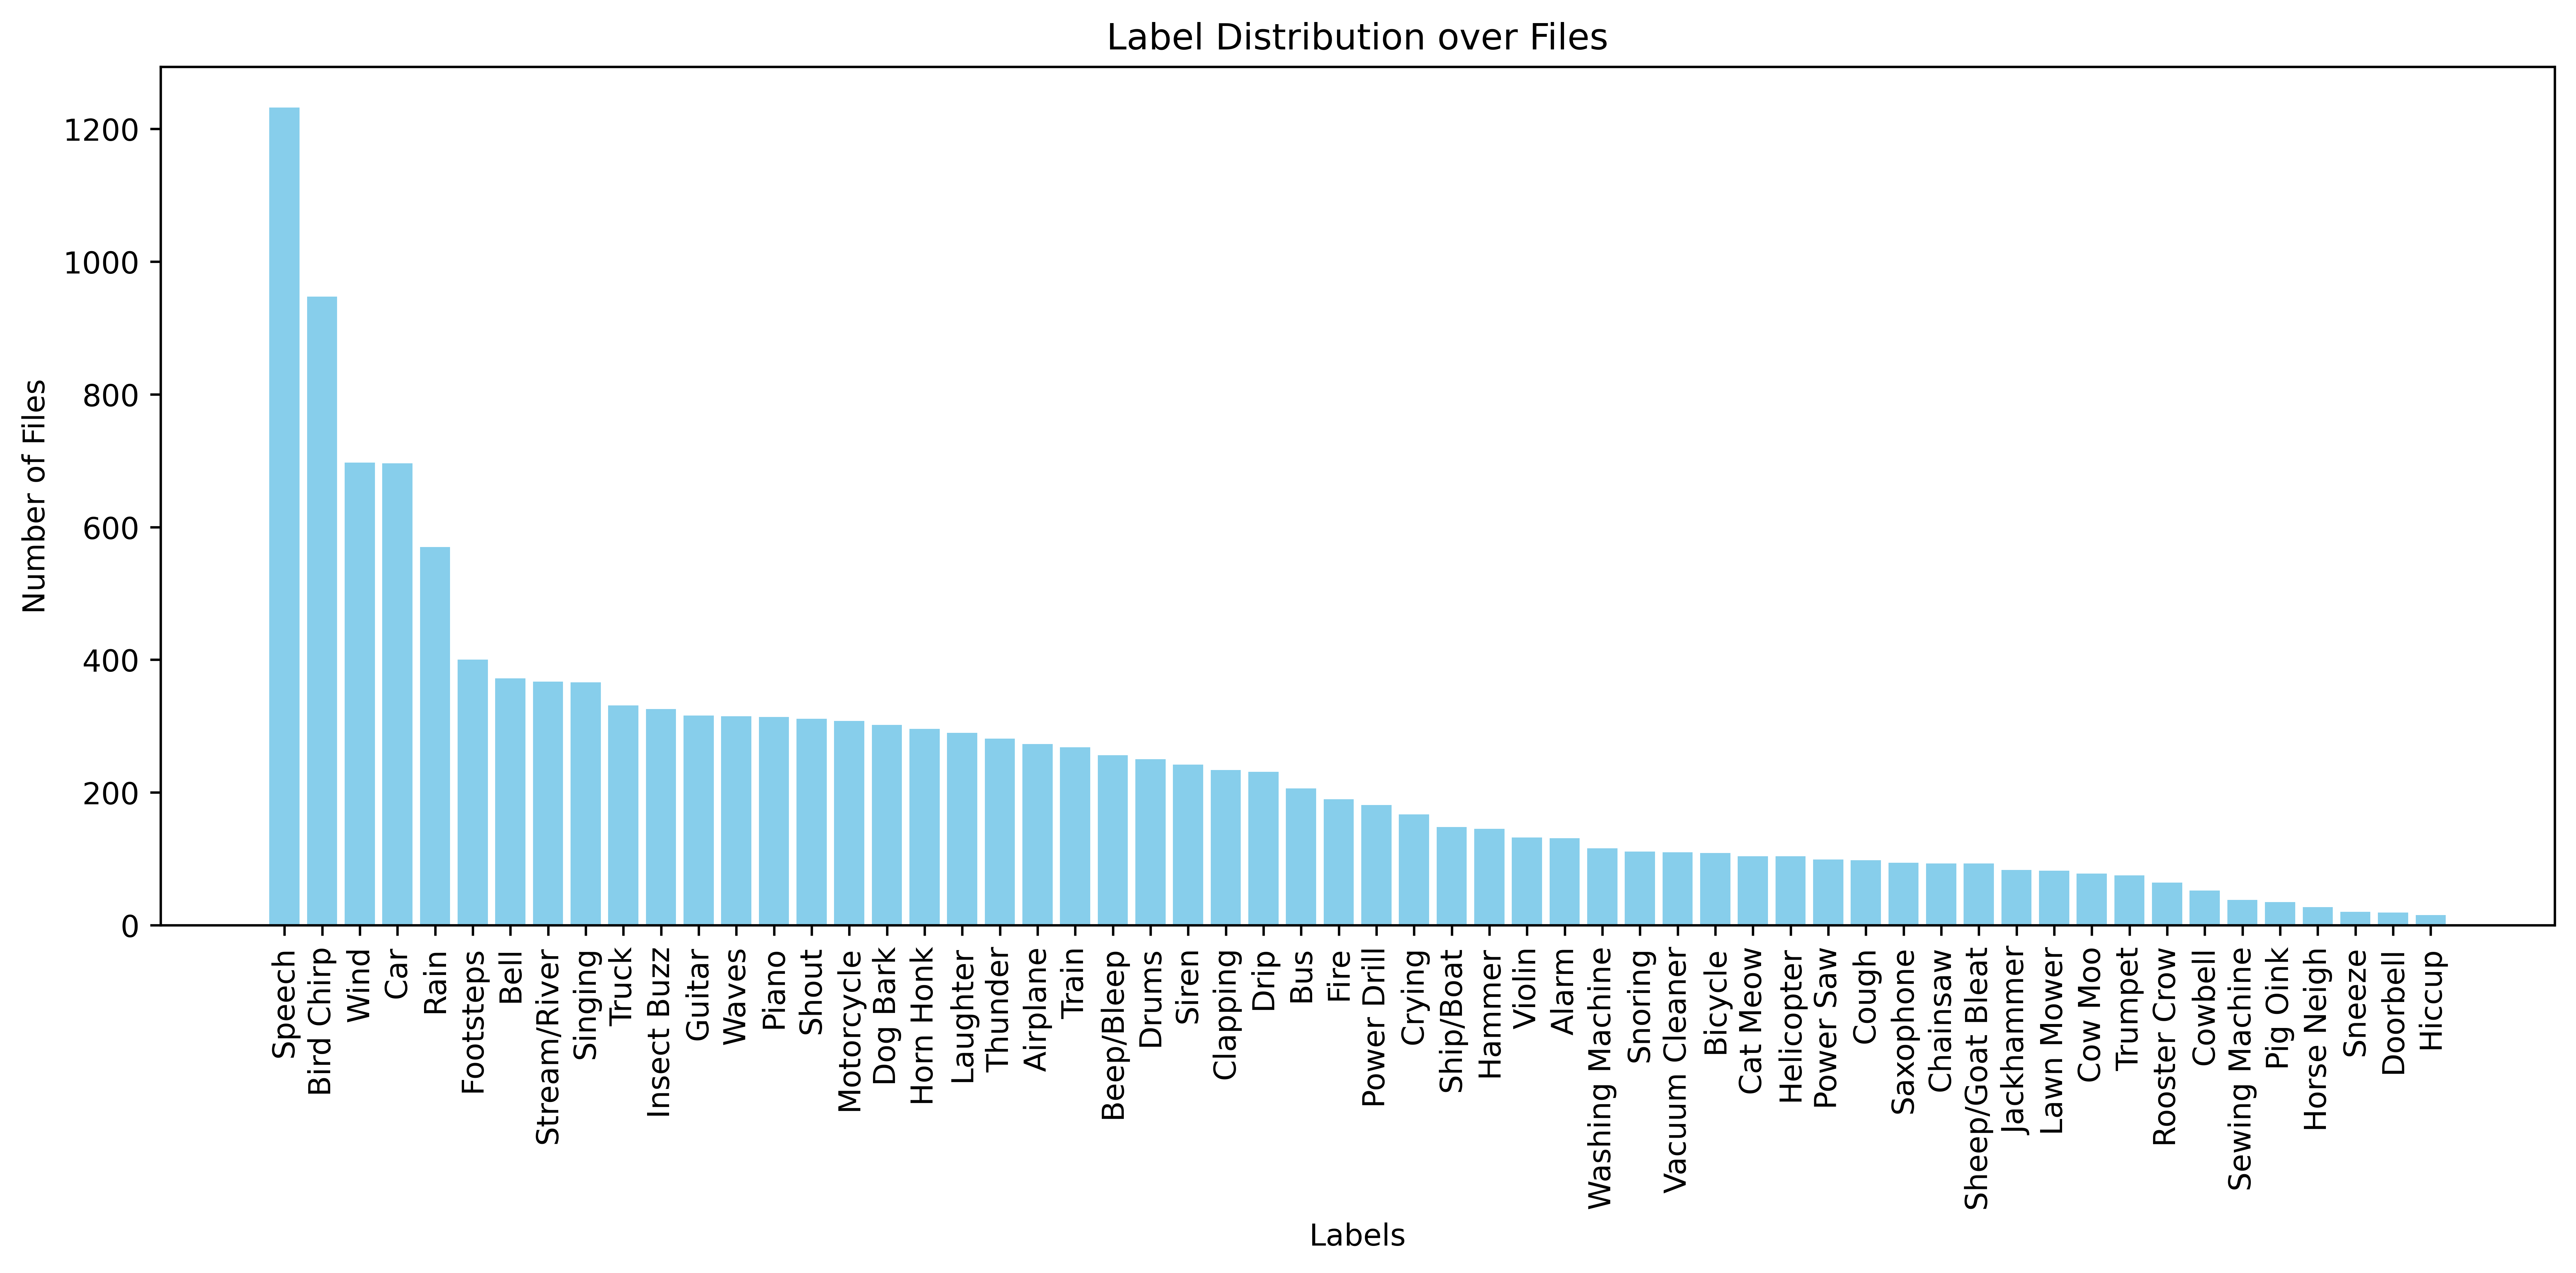
\includegraphics[width=\textwidth]{figs/2_Label Distribution over Files.png}
  \end{subfigure}
  \hfill
  \begin{subfigure}[b]{0.49\textwidth}
    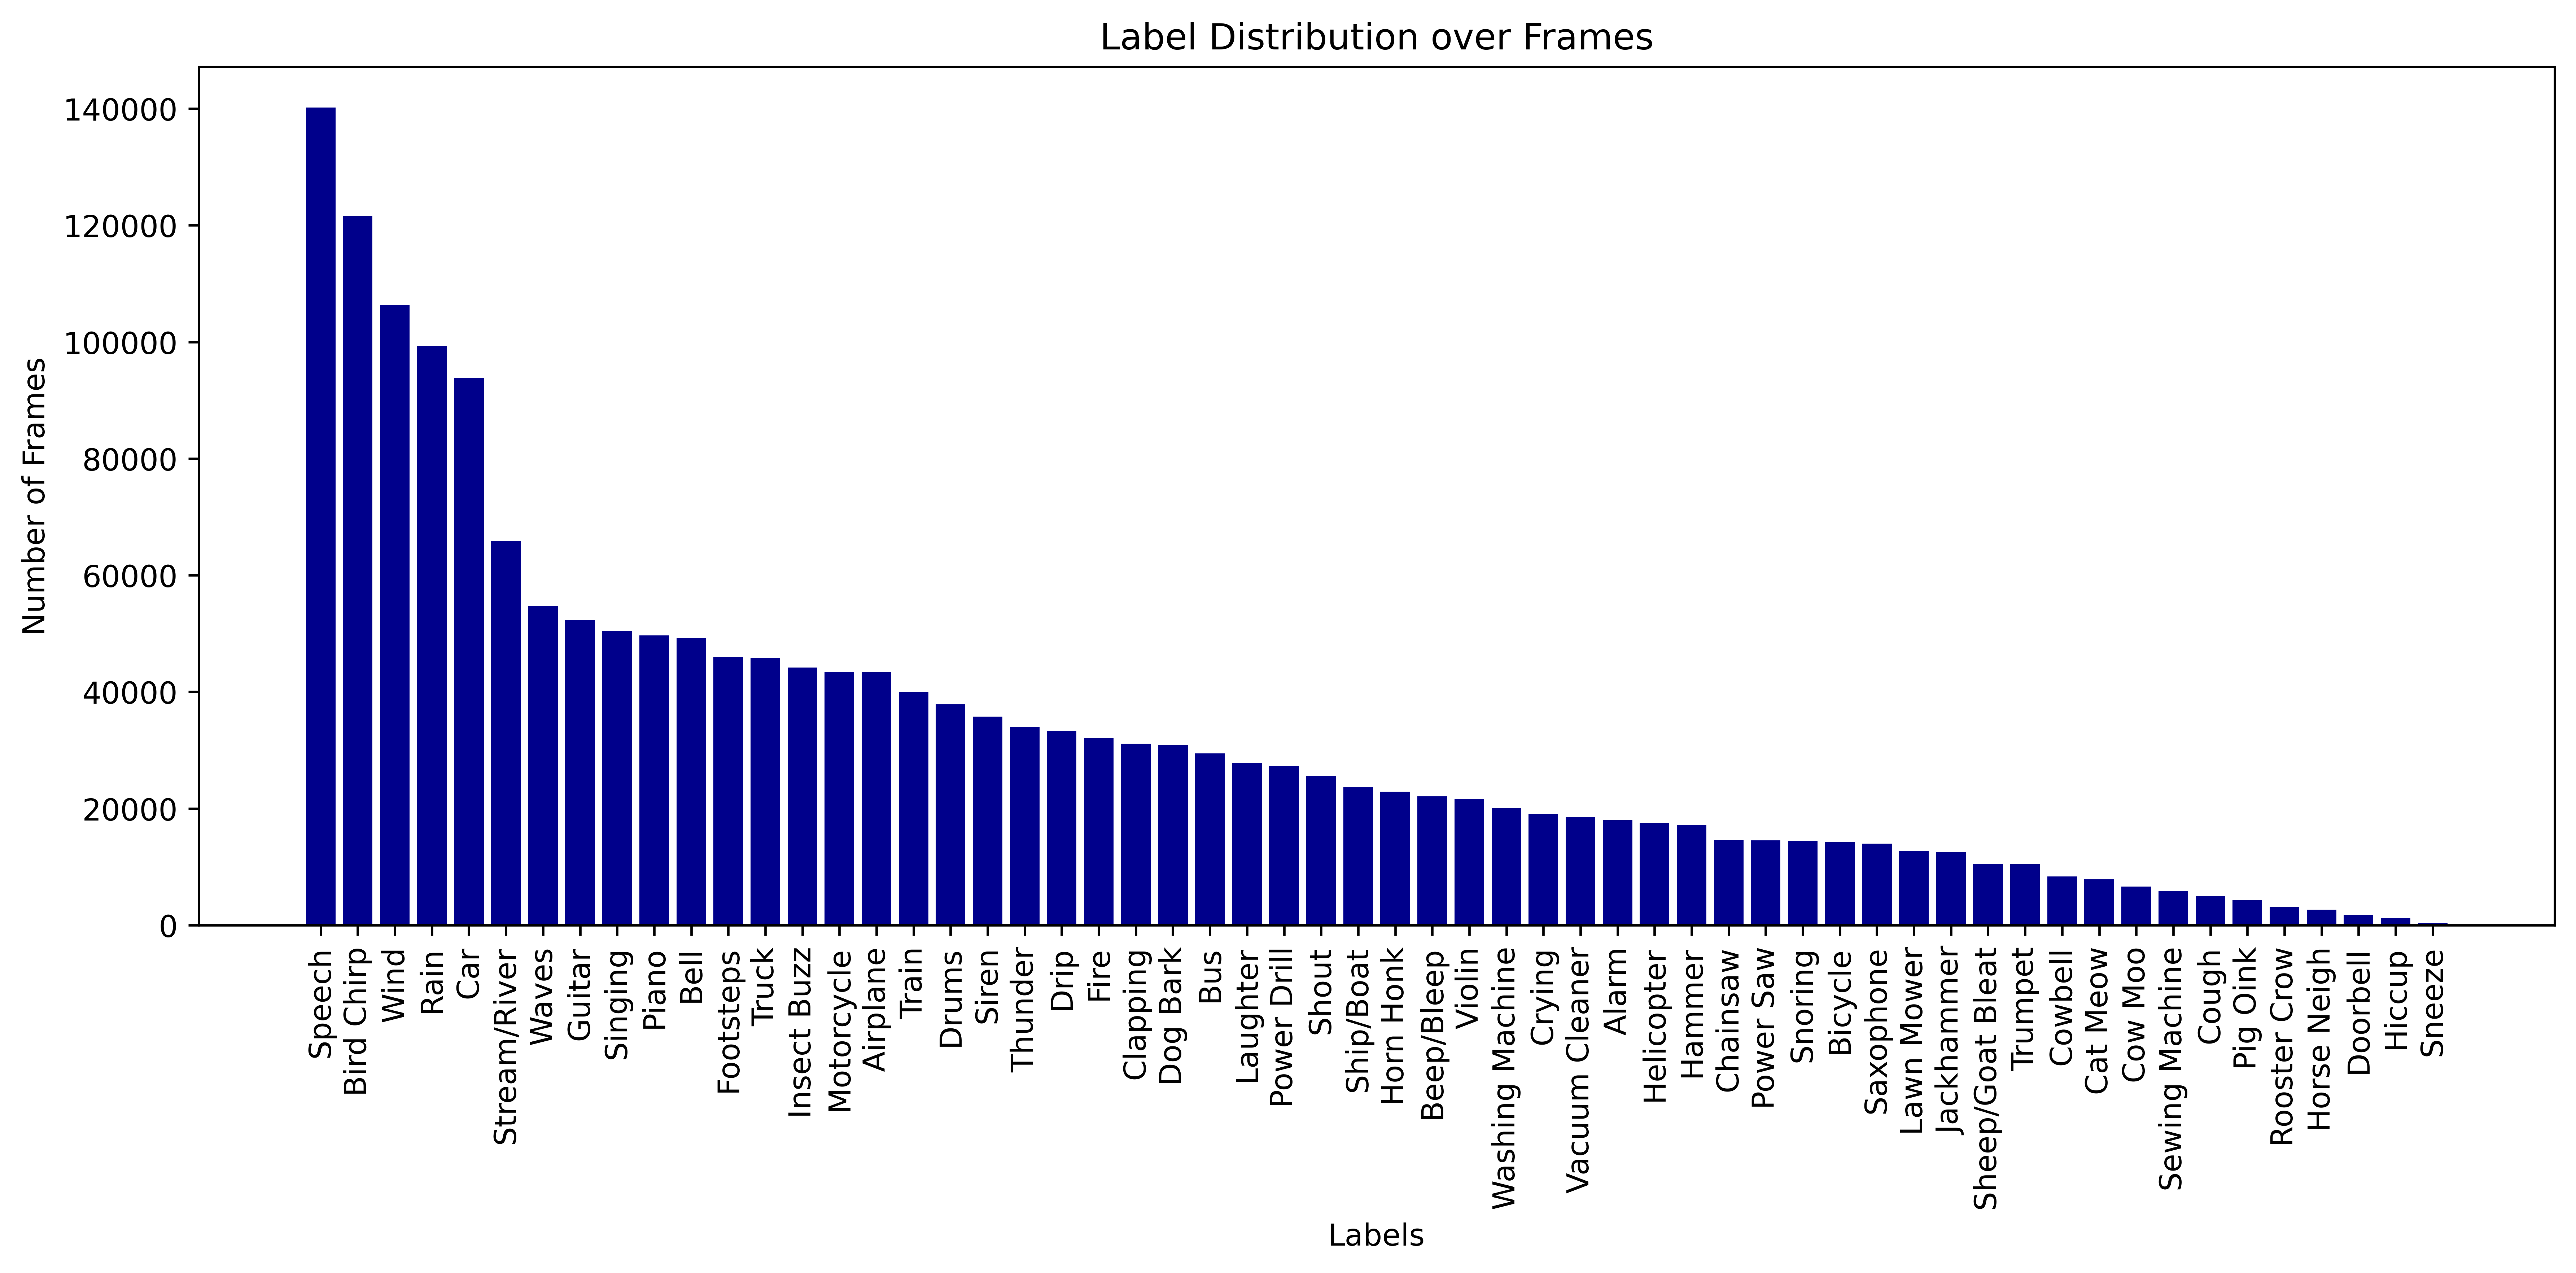
\includegraphics[width=\textwidth]{figs/2_Label Distribution over Frames.png}
  \end{subfigure}
  \caption{Label distribution}
  \label{fig:data-split}
\end{figure}



\subsection{Describe how you split the data for model selection and performance evaluation. }
\label{sec:Data Split:a}
To ensure a robust raining and proper model evaluation the available data set was independently split into three separate sets: Taring Set, Validation Set and Test set.


\begin{enumerate}
	\item {\bf Training Set: } The Training Set was used to train our classifiers. Training Set size was 60\% of our total data.
	
	\item {\bf Validation Set: } The Validation Set was used to estimate the performance of our model during training and to adjust hyperparameter, while helping us to detect potential overfitting. Validation Set size was 20\% of our total data.

	\item {\bf Test Set: } The Test Set was used to evaluate the performance of our final model and estimate how well it would perform on unseen data. This Set was unseen by our classifiers prior to the final evaluation. Test Set size was 20\% of our total data.


    
\end{enumerate}

Using Cross-Validation was considered but ultimately not used as the provided data-set was large enough to have a low risk if underfitting and produced an overall satisfying results without the implementation of Cross-Validation.


We first loaded all the audio data with the features and the labels and split it into individual frames. 



\subsection{Are there any potential factors that could cause information leakage across the data splits if they are not carefully designed? If yes, how did you address these risks?}

Yes, there are {\bf critical risks of information leakage} in audio classification if splits are not carefully designed:


\label{sec:Data Split:b}

\begin{itemize}
	\item {\bf Common Sources of Leakage: } 
    
		{\bf Temporal close audio segments: } If data is split by audio segments and not by full audio recording/session, temporal close audio segment can end up in different data sets. Because these segments will be closely related or even almost identical this would introduce data leakage to the data splits. 
        
		{\bf Same recording conditions: } If the same noise/audio source appears in both training and test sets, the model may learn source-specific features rather than class-specific ones. This can occur data from the same recording ends up in different data-sets. 

        {\bf Improper data splitting: } If data splitting is not done carefully, duplicates of the same sample might be included in multiple Sets causing data leakage.
        
        {\bf Leakage through data augmentation: } If data augmentation is applied before the data split and thus based on the entire dataset, this can result if information from the Test Set being included in the Training Set, causing leakage.\\
	
	\item {\bf Mitigation Strategies: } 
    
		{\bf File Splits:} We split the data not over the audio segments but over the full audio files. This ensures that temporally close segments and segments with the same recording condition are grouped into the same data set.

		{\bf Datasplit checking:} All data samples were indexed prior to data split and checked afterwards to ensure uniqueness among the samples. 
        
		{\bf Careful Preprocessing:} We avoided any preprocessing (e.g. feature normalization) that used statistics from the full dataset — we used only training data statistics. 
\end{itemize}


To avoid possible problems when splitting into the three data sets, 
we only split at file boundaries and tried to have an approximately equal distribution in all parts (stratification)  (\hyperref[fig:data-split]{Figure~\ref*{fig:data-split}}).
We worked in frames during pre-processing (normalization).




\subsection{Describe how you obtained unbiased final performance estimates for your models. }
\label{sec:Data Split:c}

Two main aspect were considered during model development to ensure a unbiased final performance estimation:

\begin{enumerate}
	
	\item {\bf Leakage minimization: } The prior mentioned data leakage techniques were carefully implemented to ensure a clear separation between the individual data-sets. 
    
	\item {\bf Strict Test Set Separation: } The test set was never used during training or validation. Final model evaluation was performed only once on the Test Set after all model development was completed.

%		If cross-validation is used, it’s done within the training+validation data.
%	
%	\item {\bf Repeated Experiments: } If randomness (e.g. in weight initialization or data sampling) affects results, the experiment is repeated with different seeds and the average + standard deviation is reported.
%
%	\item {\bf Stratified Sampling: } Ensures that the class distribution in all sets reflects that of the full dataset, which is particularly important in our case (unbalanced data sets).
\end{enumerate}




